\chapter{Introduzione}
\label{cap:introduzione}

Questo capitolo introduce il lavoro svolto in questa tesi, a partire dal contesto applicativo che ne motiva il problema, illustrato attraverso un esempio di riferimento, e dalla discussione dei principali filoni di ricerca correlati. Nell'introduzione del problema affrontato, se ne argomenta la non banalità e si illustrano gli obiettivi e i contributi della tesi, prima di chiudere con una descrizione dell'organizzazione dei capitoli successivi.

% ------------------------------------------------------------ %

\section{Contesto e Motivazioni}
\label{sec:contesto}

I dati sono oggi al centro di gran parte delle attività di calcolo di organizzazioni pubbliche e private, e con essi è cresciuta l'esigenza di renderli utilizzabili da soggetti diversi da chi li detiene. Un modo per farlo senza cederli è invertire il verso dello scambio: anziché consegnare i dati a coloro che vogliono elaborarli, si consente a questi ultimi di eseguire le proprie computazioni là dove i dati risiedono. Il dato quindi non lascia mai l'infrastruttura di chi lo possiede, e ciò che si sposta è la computazione. Questo approccio poggia su infrastrutture distribuite, tipicamente cluster composti da più nodi, che possono trovarsi in luoghi diversi e offrire garanzie diverse, e produce una situazione in cui la stessa infrastruttura ospita dati di natura eterogenea ed elaborazioni sottomesse da soggetti tra loro indipendenti, talvolta in concorrenza.

Per fissare le idee si consideri un esempio concreto, schematizzato in Figura~\ref{fig:esempio_contesto}. Un'organizzazione raccoglie e conserva nel tempo grandi volumi di dati, come informazioni di mercato, misurazioni provenienti da sensori o dati di mobilità e traffico urbano, e li mette a disposizione di diversi enti esterni interessati a elaborarli. Nessuno di questi soggetti entra mai in possesso dei dati grezzi, ma ciascuno si limita a sottomettere all'organizzazione un task, ovvero una computazione che dichiara di quali dataset ha bisogno per poter essere eseguita, lasciando all'organizzazione il compito di farla girare all'interno della propria infrastruttura e ottenendone in cambio soltanto l'esito, come ad esempio il risultato di un'analisi statistica o un modello addestrato su quei dati. L'infrastruttura dell'organizzazione è costituita da un cluster di nodi di calcolo, ognuno dei quali ospita localmente una parte dei dataset e si distingue dagli altri per alcune caratteristiche proprie, come il luogo in cui si trova o il grado di protezione che può garantire ai dati che vi vengono elaborati.

\begin{figure}[htb]
    \centering
    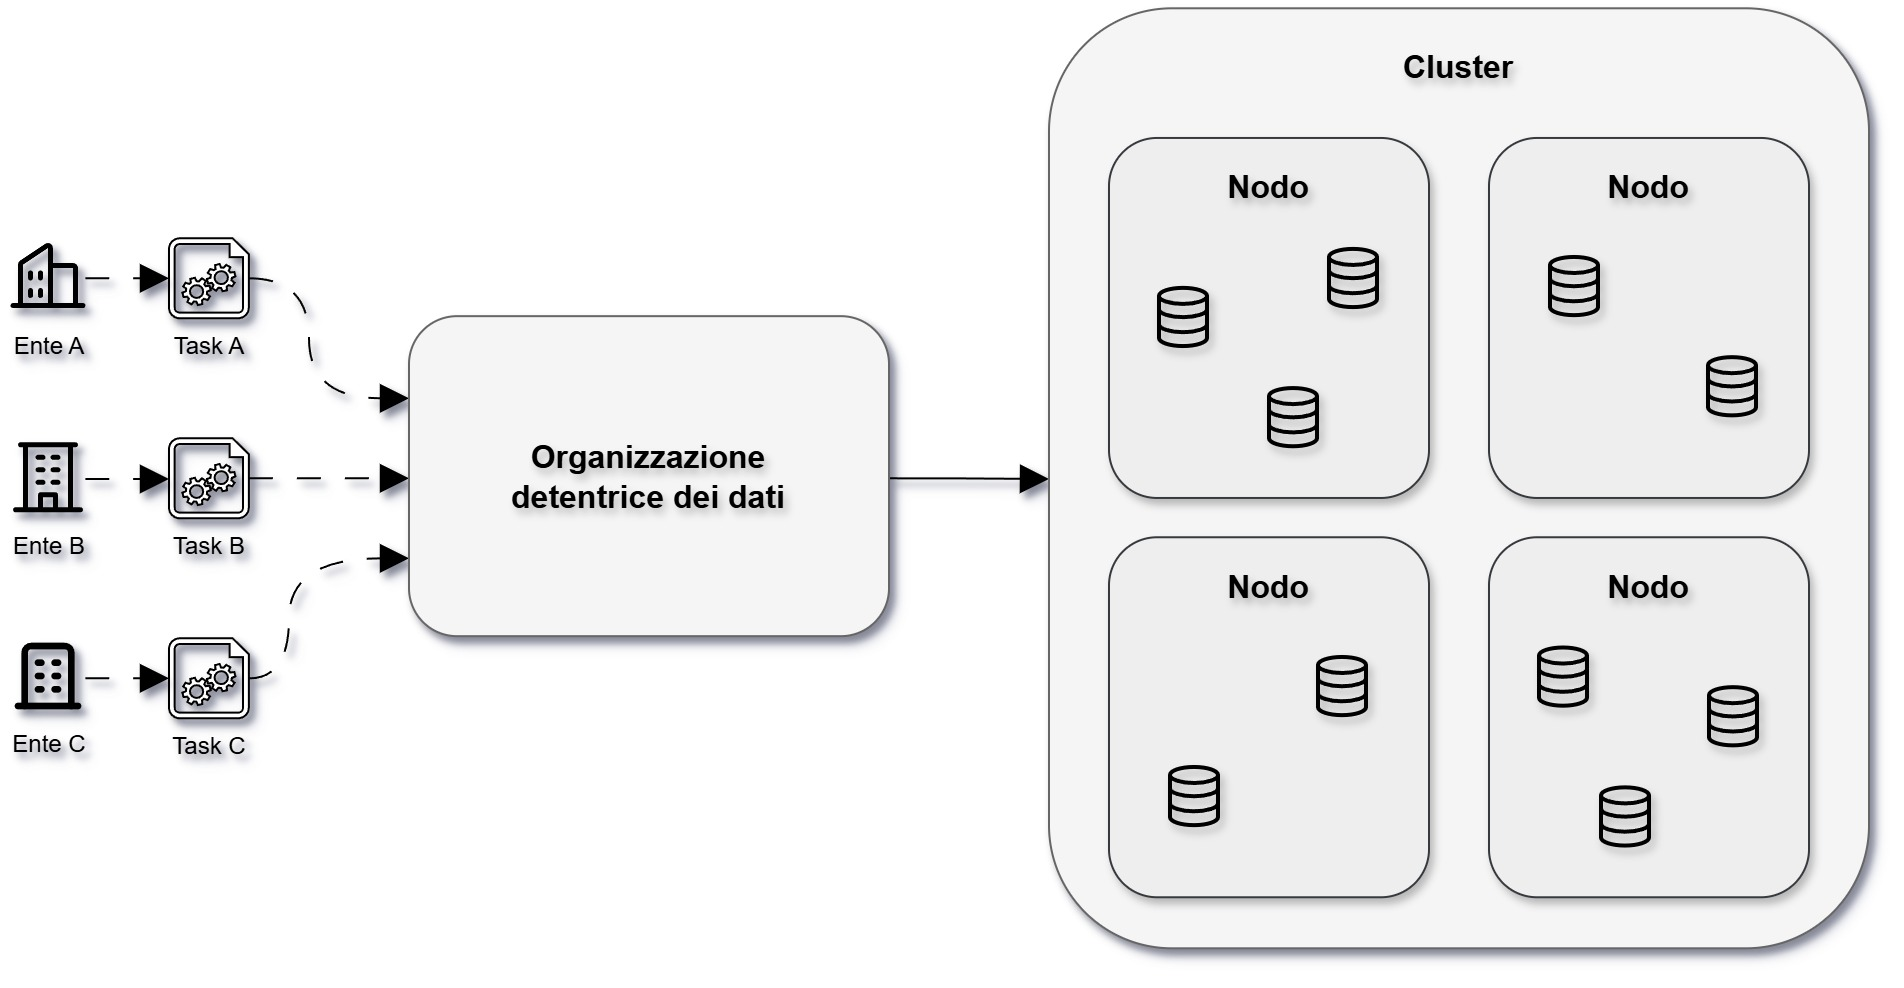
\includegraphics[width=\textwidth]{immagini/esempio.jpg}
    \caption{Enti esterni sottomettono task a un'organizzazione che detiene i dati, distribuiti sui nodi di un cluster.}
    \label{fig:esempio_contesto}
\end{figure}

A prima vista il compito dell'organizzazione potrebbe sembrare semplice, ovvero ricevere un task e mandarlo in esecuzione su un nodo che disponga dei dati richiesti e delle risorse necessarie, ma in realtà ogni richiesta porta con sé un insieme di vincoli che vanno ben oltre la semplice disponibilità di dati e risorse, e che nascono piuttosto dalla natura dei dati coinvolti. Alcuni dataset potrebbero contenere informazioni personali o comunque sensibili, sottoposte a normative come il GDPR che regolano in quali territori possano essere conservate ed elaborate, e un task che li utilizza non potrebbe quindi essere eseguito ovunque; altri, invece, potrebbero richiedere che il nodo su cui vengono trattati offra garanzie di sicurezza adeguate. Quando poi i dati necessari non si trovano già sul nodo scelto, occorre chiedersi se sia lecito farli trasferire e quanto costi farlo, tenendo presente che per alcuni di essi lo spostamento potrebbe essere del tutto escluso.

C'è infine un aspetto meno evidente, legato a ciò che accade una volta terminata l'esecuzione di un task. Un'elaborazione non scompare del tutto alla sua conclusione, ma può lasciare sul nodo che l'ha ospitata delle tracce residue dei dati utilizzati, le quali assumono particolare importanza quando i soggetti che si alternano su quel nodo sono in concorrenza tra loro. Se, ad esempio, l'ente A e l'ente B operano nello stesso settore e un task di A viene eseguito su un nodo che ha appena trattato dati riservati di B, si apre un potenziale canale di esposizione tra i due, anche in assenza di qualunque errore o comportamento scorretto da parte dell'organizzazione. Ne segue che la scelta del nodo non può basarsi soltanto su come quel nodo è fatto, ma deve tenere conto anche di ciò che vi è stato eseguito in precedenza.

Lo scenario appena descritto non è legato a un caso particolare, e le stesse esigenze si potrebbero ritrovare in contesti molto diversi tra loro. Ad esempio, un consorzio di ospedali che raccoglie e conserva i dati clinici dei propri pazienti può metterli a disposizione di gruppi di ricerca esterni che sottomettono analisi, con il vincolo che i dati non lascino l'istituto o il paese di origine; oppure un istituto finanziario che raccoglie informazioni di mercato e dati sui propri clienti può renderle disponibili a più società di consulenza esterne, alcune delle quali in concorrenza tra loro, e deve allora garantire che le informazioni di clienti concorrenti restino separate; oppure ancora un'infrastruttura di ricerca scientifica su larga scala, che raccoglie dati da più osservatori o strumenti, può dover rispettare sia vincoli di riservatezza legati a chi li finanzia sia l'impossibilità pratica di spostare i volumi più ingenti, per cui i gruppi di ricerca esterni sottomettono le proprie computazioni, che vengono eseguite direttamente dove i dati già si trovano. 

In tutti questi casi cambiano i dati, gli attori e le normative di riferimento, ma il problema di fondo resta lo stesso, rimanendo indipendente dal dominio applicativo: decidere su quale nodo distribuire una computazione che richiede determinati dati, rispettando l'insieme di vincoli che li riguardano. Per questo motivo, la soluzione sviluppata in questa tesi non è pensata per un singolo caso d'uso, ma per poter essere adattata a ciascuno di questi contesti definendo di volta in volta le regole che lo governano.

Tuttavia, una decisione come quella appena descritta non può essere lasciata a chi sottomette la richiesta. Gli enti esterni non hanno visibilità sull'infrastruttura, non sanno dove si trovino i dataset né quali nodi siano adatti ad accogliere la loro computazione, e non sarebbe nemmeno opportuno che potessero influenzarne la scelta, dato che sono proprio loro i soggetti da cui i dati vanno protetti. Le regole devono quindi essere stabilite da chi detiene i dati e applicate in modo uniforme a ogni richiesta, senza fare affidamento sulla correttezza di chi la invia. Questa tesi affronta il problema proponendo un insieme di politiche definite a livello di sistema, che stabiliscono quali assegnazioni siano ammissibili e quali tra queste siano preferibili, dandone prima una descrizione formale rigorosa, per poi realizzarle concretamente all'interno di un'infrastruttura reale.

% ------------------------------------------------------------ %

\section{Lavori Correlati}
\label{sec:stato_arte}

Il problema affrontato in questa tesi tocca diversi filoni di ricerca, ciascuno dei quali ne coglie un aspetto distinto. Da un lato ci sono vincoli normativi, come quelli legati alla \emph{data sovereignty} e alla geo-localizzazione dei dati, che impongono di tenere conto della posizione dei nodi quando si decide dove eseguire una computazione; dall'altro la \emph{data locality} guarda al problema da un'angolazione opposta, suggerendo di avvicinare il calcolo ai dati per contenerne il costo di trasferimento. A questi si affiancano i modelli formali per la gestione \emph{security-aware} delle risorse in scenari distribuiti, e il fenomeno della \emph{data remanence}, che insieme al modello \emph{Chinese Wall} guida la protezione dalle tracce lasciate dall'elaborazione, isolando tra loro esecuzioni successive in conflitto di interesse. Chiudono il quadro i lavori sullo scheduling \emph{policy-driven} in Kubernetes, che costituiscono il riferimento implementativo più vicino.

Questi aspetti vengono generalmente trattati in modo separato, mentre il contributo di questa tesi si colloca proprio alla loro intersezione. Le sottosezioni seguenti li ripercorrono singolarmente, chiarendo per ciascuno cosa viene ripreso e cosa invece cambia nell'impostazione di questa tesi.

% ------------------------------------------------------------ %

\subsection{Data Sovereignty e Geo-Localizzazione dei Dati}
\label{subsec:sovranita_dati_correlati}

Tra i vincoli che gravano sui dati, quelli legati alla sovranità sono forse i più importanti: il concetto di sovranità del dato, nella maggior parte dei casi, ruota attorno all'idea di un controllo effettivo sul luogo e sulle modalità con cui le informazioni possono essere conservate ed elaborate~\cite{data-sovereignty-review}. Le normative traducono questa esigenza in obblighi sempre più stringenti di localizzazione, che spesso non si limitano a chiedere una copia locale ma vietano il trasferimento all'estero~\cite{oecd-data-localisation}, facendo diventare così la collocazione delle risorse un problema di conformità. Rispetto a ciò, diversi lavori hanno proposto strategie di collocazione dei dati sensibili alla posizione geografica e alle regolamentazioni vigenti~\cite{geolocation-aware-data-placement, location-aware-data-placement}. Però, il focus di queste proposte resta il \emph{dove risiedono} i dati; il problema affrontato in questa tesi riguarda invece il \emph{dove eseguire} le computazioni che utilizzano quei dati, portando gli stessi vincoli dentro il processo di scheduling.

% ------------------------------------------------------------ %

\subsection{Data Locality e Costo di Trasferimento}
\label{subsec:data_locality_correlati}

La \emph{data locality} ribalta invece la prospettiva iniziale: al posto di muovere i dati verso la computazione, si avvicina la computazione ai dati. Lo scheduling nei cluster data-intensive tende a privilegiare i nodi che già ospitano gli input richiesti, accettando anche di ritardare l'avvio di un task pur di eseguirlo vicino ai dati, per poter ridurre il traffico della rete~\cite{delay-scheduling, data-locality-investigation-mapreduce}. Lo stesso principio guida gli approcci di \emph{near-data processing}~\cite{beyond-the-wall-ndp}, che eseguono parte dell'elaborazione direttamente accanto alla memoria in cui i dati risiedono, e più in generale lo scheduling che assegna la computazione al nodo dove i suoi dati sono già presenti, così da non doverli spostare sulla rete~\cite{transfer-cost-aware-edge-scheduling}. In tutti questi casi eseguire vicino ai dati è una scelta che conviene ma non un obbligo, mentre in altri diventa l'unica strada percorribile: quando i volumi rendono impraticabile qualsiasi spostamento~\cite{bringing-computation-moea}, o quando certi dataset non possono in alcun modo lasciare il nodo in cui risiedono, e allora è la computazione a doversi spostare verso i dati, dato che questi ultimi non possono essere trasferiti~\cite{paradigm-non-transferable-dataset}. Rispetto a ciò, questa tesi eredita l'ottimizzazione del costo di trasferimento, mentre la non trasferibilità di alcuni dataset non entra come semplice costo da minimizzare, ma come una condizione che esclude a priori i nodi che non possono ospitarli. 

% ------------------------------------------------------------ %

\subsection{Modelli Formali per la Gestione Security-Aware delle Risorse}
\label{subsec:modelli_formali_correlati}

Più vicini allo spirito di questa tesi sono i modelli formali per la gestione \emph{security-aware} delle risorse in scenari cloud e multicloud. Il riferimento principale, da cui questo lavoro trae la propria impostazione, è un modello per l'allocazione di dati soggetti a requisiti di protezione~\cite{sec-aware-data-alloc-multicloud}, nel quale i servizi cloud disponibili vengono classificati rispetto a proprietà di sicurezza astratte, ciascuna con livelli ordinati definiti da condizioni sugli attributi concreti del servizio, mentre ogni risorsa da collocare dichiara la classe minima che il servizio deve garantire per poterla ospitare. Il modello proposto in questa tesi riprende questa struttura e la adatta a un altro contesto: a essere classificati per proprietà astratte sono i nodi del cluster, e a dichiarare requisiti su di essi sono sia i task da eseguire sia i dataset che questi consumano, così che l'ammissibilità di un nodo nell'ospitare un task diventa un confronto tra livelli nello stesso spazio in cui i nodi sono classificati. Nella stessa direzione si colloca anche il lavoro sul supporto ai requisiti di sicurezza nella gestione delle risorse cloud~\cite{supp-sec-req-res-management-cloud}, dove le esigenze di protezione espresse dalle parti coinvolte si traducono in vincoli sull'allocazione. 

Un'ulteriore fonte di ispirazione sono le metodologie per la selezione dei piani cloud~\cite{supporting-user-requirement-pref-cloud, cloud-plan-selection-req-multiple-app}, che valutano e classificano le alternative disponibili sulla base di molteplici requisiti e delle preferenze espresse dagli utenti; ne deriva l'idea che, tra le opzioni ammissibili, la scelta finale combini più criteri di valutazione. Da tutto questo, il modello proposto eredita due idee: descrivere i nodi per proprietà astratte su cui le entità esprimono i propri requisiti, e valutare le alternative ammissibili secondo criteri multipli. Cambia però l'oggetto della decisione, perché nei casi citati si stabilisce dove collocare i dati o quale piano scegliere, mentre qui si stabilisce a quale nodo affidare la computazione, portando gli stessi strumenti formali dentro il processo di scheduling, dove l'ammissibilità del nodo e il costo di accesso ai dati richiesti entrano nella decisione stessa e non a valle di essa.

% ------------------------------------------------------------ %

\subsection{Data Remanence e Isolamento tra Elaborazioni}
\label{subsec:chinese_wall_correlati}

Finora i vincoli considerati riguardano principalmente il luogo in cui i dati possono essere conservati o raggiunti dalla computazione. Però, come anticipato nella Sezione~\ref{sec:contesto}, anche ciò che accade dopo l'elaborazione è rilevante, dato che l'esecuzione di un task può lasciare sul nodo tracce dei dati utilizzati. Il fenomeno prende il nome di \emph{data remanence}, ed è documentato sia come problema generale in ambito cloud~\cite{survey-data-remanence-cloud}, sia a livello dei supporti fisici di memorizzazione~\cite{data-remanence-flash-memory}, dove frammenti dei dati o della loro elaborazione possono sopravvivere in memoria, nello storage effimero o nelle cache anche dopo la fine dell'esecuzione. In un nodo condiviso tra soggetti in concorrenza, questo residuo diventa il punto in cui potrebbe nascere un conflitto di interesse.

Il riferimento naturale per questo tipo di problema è il modello \emph{Chinese Wall} di Brewer e Nash~\cite{chinese-wall-brewer-nash}, nato in ambito finanziario per impedire che un soggetto acceda a informazioni di aziende in conflitto tra loro, erigendo un muro che gli vieta ogni accesso ulteriore ai concorrenti di chi ha già consultato. Dal modello originale sono poi nate diverse varianti che ne approfondiscono la memoria del soggetto e ne modificano la logica, rimettendo in discussione, ad esempio, la transitività della relazione di conflitto~\cite{chinese-wall-aggressive-lin}. Proprio tra queste osservazioni emerge un limite noto del modello classico: una volta costruito, un muro non viene mai rimosso, e l'assenza di un meccanismo che ne preveda il decadimento prima o poi porta inevitabilmente ogni soggetto a restare bloccato dai propri accessi passati~\cite{chinese-wall-kessler}. Questa tesi adotta questo principio di isolamento sull'asse nodo-task, applicandolo alla relazione tra un nodo condiviso e le esecuzioni di task che vi si susseguono, così come è già stato fatto ad esempio per l'isolamento fisico tra macchine virtuali in conflitto ospitate sullo stesso nodo di un'infrastruttura cloud~\cite{chinese-wall-cloud-nodes-data}, con un'inversione di prospettiva rispetto alla memoria di cui parla il modello classico, che per una persona fisica è la rappresentazione della sua conoscenza accumulata, mentre per un nodo di calcolo è un componente fisico concreto. Lo stato lasciato dalle elaborazioni passate entra così a pieno titolo nelle politiche di isolamento tra nodi e task, offrendo allo stesso tempo una via d'uscita dalla \emph{starvation} che nel modello originale restava un problema aperto; questo perché, a differenza della memoria di una persona, quella di un nodo può essere ripulita, rimuovendo materialmente le tracce delle elaborazioni precedenti e facendo così decadere il muro che esse avevano imposto.

% ------------------------------------------------------------ %

\subsection{Scheduling Policy-Driven in Kubernetes}
\label{subsec:k8s_correlati}

Passando alla parte implementativa, il riferimento più diretto è dato da due lavori sullo scheduling \emph{policy-driven} in Kubernetes~\cite{policy-driven-sec-aware-scheduling-k8s, secure-k8s-workload-deployment}. Il problema da cui partono è che i vincoli di selezione del nodo vanno scritti a mano nella specifica di ogni singolo \texttt{Pod}, con il rischio di configurazioni fragili e soggette a errori; la loro proposta consiste nel definire le politiche una volta sola a livello di cluster e affidarne l'applicazione automatica a OPA Gatekeeper, che in fase di ammissione traduce etichette di alto livello nei vincoli di scheduling corrispondenti e rifiuta le richieste che violano le politiche stabilite, con un impatto trascurabile sulle prestazioni. Con questi lavori la tesi condivide l'impostazione di fondo, ovvero governare lo scheduling tramite politiche definite centralmente e realizzarlo sui meccanismi di estensione di Kubernetes, riprendendone l'uso di OPA Gatekeeper per la validazione delle richieste. Però, il loro intervento si limita alla fase di ammissione, dopo la quale la scelta del nodo resta allo scheduler nativo, che si basa su vincoli fissati una volta per tutte al momento della creazione del \texttt{Pod}~\cite{k8s-scheduler}. Per il problema affrontato qui questo non basta, perché assieme alle politiche statiche di questo tipo servono anche politiche dinamiche, come quella di isolamento ispirata alla Chinese Wall precedentemente discussa, che dipendono dallo stato che un nodo ha accumulato nel tempo, oltre ad altri criteri come il costo di accesso ai dati richiesti: condizioni dinamiche di questo genere non possono essere fissate in ammissione e vanno valutate nel momento stesso in cui un nodo viene scelto. Ne consegue la necessità di estendere anche lo scheduler nativo di Kubernetes, portando la logica delle politiche fino alla fase di scheduling vera e propria~\cite{k8s-scheduler-framework}.

% ------------------------------------------------------------ %

\section{Obiettivi e Contributi}
\label{sec:obiettivi}

Il problema delineato nella Sezione~\ref{sec:contesto} potrebbe apparire come una semplice variante dello scheduling tradizionale, ma diversi elementi lo rendono tutt'altro che banale. Il primo è che i vincoli provengono da fonti diverse e vanno soddisfatti simultaneamente, senza che esista un ordine naturale in cui valutarli; le caratteristiche richieste dal task, i requisiti di protezione di ciascun dataset, i limiti geografici imposti dalle normative e l'ammissibilità di un eventuale trasferimento si combinano tra loro, e talvolta spingono in direzioni opposte, come accade quando la convenienza di eseguire un task vicino ai propri dati si scontra con un nodo che, pur ospitandoli, non offre le garanzie richieste. Il secondo è che una parte di questi vincoli non dipende soltanto da come un nodo è fatto, ma da ciò che è accaduto in passato, vincolando quindi la decisione a uno stato che evolve a ogni assegnazione e che va periodicamente ripristinato, per evitare che i nodi finiscano per diventare inutilizzabili. Il terzo riguarda la separazione delle responsabilità precedentemente discussa, secondo cui chi sottomette un task è proprio il soggetto da cui i dati vanno protetti, e per questo non ci si può affidare allo stesso per indicare i vincoli da rispettare, ma è il sistema a doverli applicare uniformemente a ogni richiesta. L'ultimo, non per importanza, è che tutto questo deve poter essere realizzato all'interno di un orchestratore reale, i cui meccanismi nativi non prevedono né vincoli legati alla protezione dei dati né decisioni che dipendano dallo stato accumulato dai nodi.

L'obiettivo del lavoro è quindi progettare e realizzare un sistema di scheduling \emph{policy-driven} per task che consumano dataset soggetti a vincoli di protezione, con due contributi principali. Da una parte un modello formale che descrive matematicamente le entità coinvolte, le politiche che ne governano i vincoli e il criterio con cui individuare il nodo migliore tra quelli ammissibili, riprendendo dalla letteratura le idee usate per la distribuzione dei dati e la selezione delle risorse e adattandole alla distribuzione della computazione, con l'aggiunta di una politica di isolamento ispirata al modello \emph{Chinese Wall}, che tiene conto della storia delle elaborazioni su ciascun nodo. Dall'altra l'implementazione del modello in ambiente Kubernetes, sfruttando i meccanismi di estensione nativi per portare la valutazione delle politiche dalla fase di ammissione delle richieste fino alla scelta effettiva del nodo.

% ------------------------------------------------------------ %

\section{Organizzazione della Tesi}
\label{sec:organizzazione}

Il resto dei capitoli di questa tesi va dalla definizione del problema alla sua realizzazione concreta. Il Capitolo~\ref{cap:definizione} inquadra lo scenario applicativo e gli attori coinvolti, fissa le assunzioni entro cui il sistema opera e introduce la formalizzazione dei concetti di base, per poi enunciare le proprietà che il sistema garantisce per costruzione. Il Capitolo~\ref{cap:modello} costituisce il nucleo teorico della tesi, dove si sviluppa il modello di scheduling policy-driven, dalla classificazione dei nodi per proprietà astratte alla compatibilità tra requisiti delle entità e caratteristiche dei nodi, passando per i vincoli geografici, la staticità dei dataset e il costo del loro trasferimento, fino al trattamento dei conflitti di interesse tra contesti e all'isolamento dei nodi rispetto ai task, chiudendo con un esempio applicativo completo che mostra il modello all'opera. Il Capitolo~\ref{cap:implementazione} descrive come questo modello venga tradotto in un sistema funzionante in ambiente Kubernetes, sfruttando i meccanismi di estensione nativi della piattaforma per realizzare la validazione delle richieste, la loro traduzione in unità schedulabili e lo scheduler personalizzato che ne implementa filtraggio e ottimizzazione. Il Capitolo~\ref{cap:valutazione} raccoglie la valutazione sperimentale del sistema, concentrandosi sulla componente dinamica il cui comportamento dipende dallo stato del cluster, e ne analizza l'impatto sulla latenza di scheduling al variare del grado di conflitto e della frequenza di sanificazione dei nodi. Infine, il Capitolo~\ref{cap:conclusioni} trae le conclusioni del lavoro svolto alla luce di quanto emerso lungo l'intero elaborato, discutendone le possibili direzioni di sviluppo future.